\setlength{\footskip}{8mm}

\chapter{METHODOLOGY}\label{methodology}

\section{Study 1: Confirming the parameters}\label{metho-s1}

The goal of this study is to determine how measurement locations and schemes impact Raman spectra.
The findings of this study will be utilized to plan the experiment in section.~\ref{metho-s2}.

\subsection{Equipment}
The Raman instrument, which includes a 785 nm laser and a 10x objective lens, will be utilized to evaluate the Raman spectra.
The Accu-Chek® Guide Meter is a standard blood glucose meter for SMBG \citep{accu2022} and will be used to check glycemic control.

\subsection{Studying Measuring schemes}
We have previously performed the measurements on the nailfold and index fingertip, however the findings are still confusing due to variances in the specifications of our Raman instruments.
To avoid issues caused by ambiguous spectrum data, we must first check the spectral from a liquid sample (e.g., glucose solution, blood) before evaluating the Raman spectroscopy at four different locations: the wrist, forearm, index fingertip, and index nailfold.
The several measurement systems will be put to the test to discover which one gives the greatest scattering signal while avoiding fluorescence interference.
The best measurement techniques will be utilized for the remainder of the Raman scattering evaluation.


\subsection{Data collection}
The solution's spectral data will be used to measure the concentration of glucose in distilled water and blood. The Oral Glucose Concentration will regulate the glucose concentration in blood.
\\(1) Distilled water
\\(2) Glucose solution (diluted in distilled water) 70, 80, 90, 100 mg/dL for imitating normal fasting blood glucose condition.
\\(3) Glucose solution (diluted in distilled water) 110, 120, 130 mg/dL for imitating fasting blood glucose fluctuations. These concentrations indicate a proclivity for diabetes.
\\(4) Blood from participants in normal fasting blood glucose condition. (participants will be restricted to fasting for eight hours.)
\\(5)  Blood from individuals in the OGTT-controlled fasting blood glucose fluctuations condition
\\
The healthy volunteers' glucose levels will be manipulated using the Oral Glucose Tolerance Test (OGTT).
Participants must fast for at least eight hours before to the test.
After arriving at the experiment location, participants will be asked to acclimate for 30 minutes.
The instructor will repeat the experiment technique during the acclimatization period.
Data will be collected at the desired measurement point using both a Raman Instrument and conventional SMBG equipment.
When the acclimatization period is over, the first sample will be taken.
The OGTT begins with the subjects consuming a 250 ml of water containing 75 g of glucose in five minutes.
Then, over the following two hours, 
\\(1) take Raman spectra from the interesting measuring site every five minutes
\\(2) collect blood samples from the interested measuring site every 20 minutes.
\\There will be 25 Raman samples and eight blood samples in total.

Each participant has to repeat the experiment until all four measuring sites are measured. 
The experiment has to be done on another day.

\subsection{Metric}

The glucose spectra will be extracted by subtracting two Raman signals.
The remaining signal is the change in glucose concentration, as shown in the derivation below.

The Raman spectra ($\text{RS}$) contains glucose fingerprint ($\text{G}$) and tissue spectra ($\text{T}$).

\begin{equation}\label{eq:rs}
    \text{RS} = \text{G} + \text{T}
\end{equation}

Then, the subtraction of two Raman signal can be represented as follows;

\begin{equation}\label{eq:deltars}
    \Delta \text{RS} = \text{RS}_1 - \text{RS}_2
\end{equation}

where $\text{RS}_i$ is the Raman spectra measured at time $i$. 
Then, substituting Equation~\ref{eq:deltars} with Equation~\ref{eq:rs} will derive the follows

\begin{equation}
    \Delta \text{RS} = \Delta \text{G} + \Delta \text{T}
\end{equation}

Given the same measurement site, the tissue spectra will be the same.
Thus, $\Delta \text{T}$ is $0$.
Then, it is obvious that 

\begin{equation}
    \Delta \text{RS} = \Delta \text{G}
\end{equation}

As a result, the optimum measurement site is the one with the highest correlation between $\Delta \text{G}$  and real blood glucose fluctuations.

%%%%%%%%%%%%%%%%%%%%%%%%%%%%%%%%%%%%%%%%%%%%%%%%%%%%%%%%%%%%%%%%%%%%%%%%%%%%%
\section{Study 2: Raman scattering analysis of blood glucose}\label{metho-s2}

The objective of this study is to create a model of the correlation between Raman spectra and blood glucose levels.
The same equipment from section~\ref{metho-s1} will be used.
The measuring site and scheme are chosen based on the result of Section~\ref{metho-s1}.

\section{Data Collection}

The identical data collecting and experiment approach as in section~\ref{metho-s1} will be employed.
In this study, we raise the number of participants to 15.
Participants must be between the ages of 20 and 35, 36 to 50, and 51 to 65.
A total of $15 \times 25 =  375$ Raman samples and $15 \times 8 = 120$ blood samples are collected.

\section{Preprocessing and Data Modeling}

The acquired Raman spectra will be normalized by their intensity of 1450 or 1549 $\text{cm}^{-1}$.
Thus, there are three preprocessing options: (1) without normalization, (2) normalize with 1450 $\text{cm}^{-1}$, and (3) normalized with 1549 $\text{cm}^{-1}$.
The Linear Regression (LR) model will be used to assess the linearity of 1125 $\text{cm}^{-1}$ with glucose concentration.
The MLR model with 911, 1060, 1125 $\text{cm}^{-1}$ as inputs we will use for multivariate analysis.
As a baseline model, full spectrum with PLS will also be employed.

In total, there will be $3 \times 3 = 9$ combinations to compare.

\section{Metric}

The Pearson correlation will be used to evaluate the model's performance.
Furthermore, resource use during prediction will be monitored.

\section{Study 3: Designing and developing wearable blood glucose device}

\begin{figure}
    \caption{An example of wearable \citep{fitbitwatch}.}
    \centerline{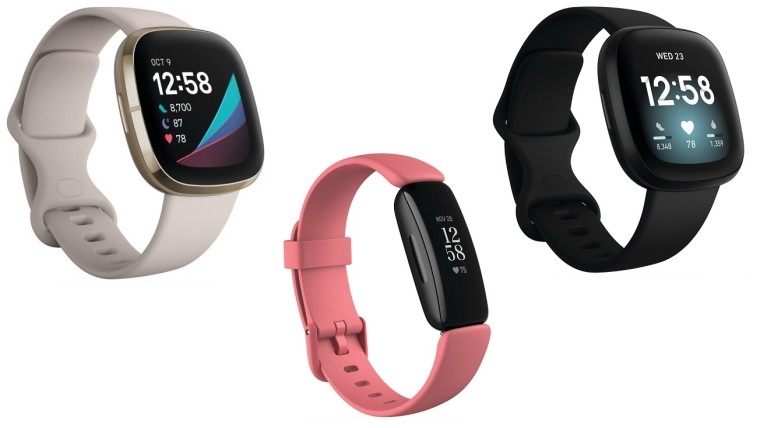
\includegraphics[width=3in]{figures/example-fitbit.jpeg}}\label{fig:fitbitwatch}
    % \small{\textit{Note.} Additional notes goes here.}
\end{figure}


\textbf{Objective}: Design and develop a prototype of a wearable SMBG.\\
% \textbf{Independent Variables}: \\
% \textbf{Dependent Variables}: \\
\textbf{Outcome}: A prototype.

\section{Study 4: Device Evaluation}

\textbf{Objective}: To evaluate the prototype, we redo Section~\ref{metho-s2} experiment with our prototype.\\
\textbf{Independent Variables}: Raman scattering of blood\\
\textbf{Dependent Variables}: Glycemic\\
\textbf{Outcome}: Prototype achieves glycemic prediction correlation $R^2 > 0.8$ with actual glycemic.
